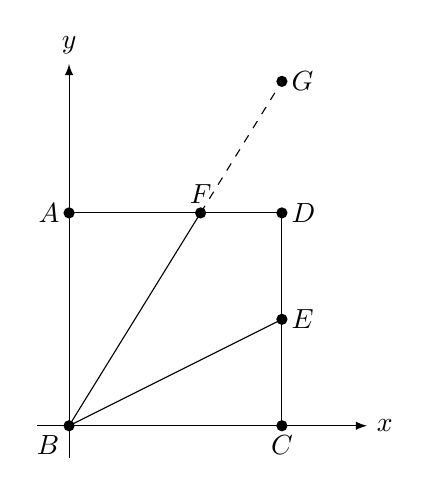
\begin{tikzpicture}[scale=1.3514,>=latex]
  \draw[->] (-0.3,0)--(2.8,0) node[right]{$x$};
  \draw[->] (0,-0.3)--(0,3.4) node[above]{$y$};
  \coordinate (B) at (0,0); \coordinate (C) at (2,0);
  \coordinate (D) at (2,2); \coordinate (A) at (0,2);
  \coordinate (E) at (2,1); \coordinate (G) at (2,3.236);
  \coordinate (F) at (1.236,2);
  \draw (A)--(B)--(C)--(D)--cycle;
  \draw (B)--(E); \draw (B)--(F); \draw[dashed] (F)--(G);
  \foreach \p/\pos in {A/left,B/below left,C/below,D/right,E/right,F/above,G/right}
    \fill (\p) circle(1.5pt) node[\pos]{$\p$};
\end{tikzpicture}
